\chapter{Onde elettromagnetiche}

\lecture{15}{16 aprile 2024}

\section{Equazione di D'Alembert}
Tra il 1863 e il 1865 Maxwell propose una teoria dell'elettromagnetismo che oggi sono sintetizzate nelle equazioni che portano il suo nome: "Equazioni di Maxwell".
\begin{figure}[H]
	\centering
	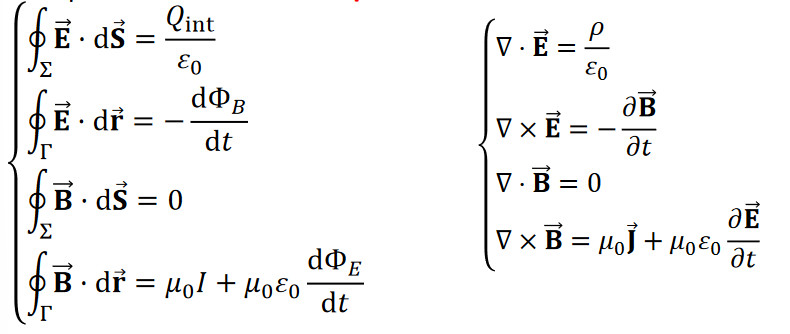
\includegraphics[width=0.5\textwidth]{screenshots/2024-04-16-11-21-47.png}
\end{figure}
\noindent dove \(Q_{int}, \rho , I, \vec{J} \)	si riferiscono a cariche e correnti vere. Ci poniamo nel vuoto:
\begin{figure}[H]
	\centering
	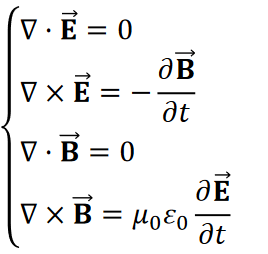
\includegraphics[width=0.2\textwidth]{screenshots/2024-04-16-11-25-38.png}
\end{figure}
Consideriamo \(\frac{\partial \vec{E}}{\partial t}\neq \vec{0} \) in un punto dello spazio. Allora il rotore del campo magnetico sarà diverso da zero. \(\nabla \times \vec{B}\neq \vec{0} \implies \vec{B}\neq \vec{0} \) in una regione spaziale infinitesima attorno a quel punto. Ma di conseguenza si genera un campo elettrico nella regione circostante di spazio. Una perturbazione locale si è propagata nello spazio circostante! Maxwell valutò che la perturbazione doveva muoversi con velocità \(v\thickapprox \SI{3.11e8}{m/s}\). La velocità della luce nota nel 1865 era \(\SI{2.98e8}{\metre \per \second} \leq v \leq \SI{3.15e8}{\metre \per \second}\). Non c'era nient'altro di vicino a quella velocità, quindi si ipotizzò che la luce potesse essere un fenomeno elettromagnetico.

Hertz fece un esperimento:
\begin{figure}[H]
	\centering
	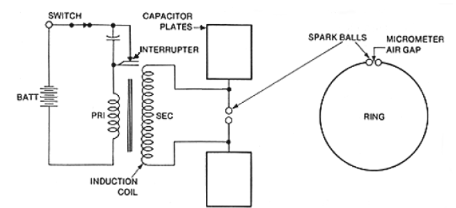
\includegraphics[width=0.5\textwidth]{screenshots/2024-04-16-11-30-59.png}
\end{figure}
La batteria genera corrente continua, attraverso il trasformatore viene trasformata in corrente alternata che carica le placche di un capacitore. Ogni tanto le sferette scaricano una scintilla e questo provoca una scintilla nel risonatore circolare che non è connesso a nulla. Augusto Righi nel 1894 produsse delle onde micrometriche, mentre Marconi nel 1895 controllò un interruttore da remoto.

Scrivendo le equazioni di Maxwell in termini di \(\vec{H}\) esse diventano più simmetriche:
\begin{figure}[H]
	\centering
	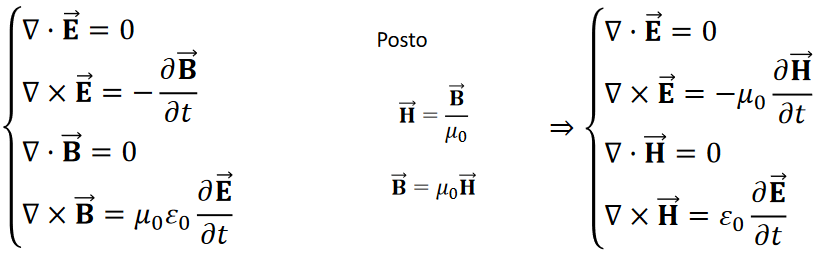
\includegraphics[width=0.5\textwidth]{screenshots/2024-04-16-11-35-50.png}
\end{figure}
Sono equazioni differenziali alle derivate prime, lineari e omogenee. Di conseguenza vale il principio di sovrapposizione. Ricaviamo l'equazione di D'Alembert per le onde elettromagnetiche. Ricordando che \(\curl (\curl \vec{v}) = \grad(\div \vec{v})- \laplacian{\vec{v}} \), otteniamo:
\begin{figure}[H]
	\centering
	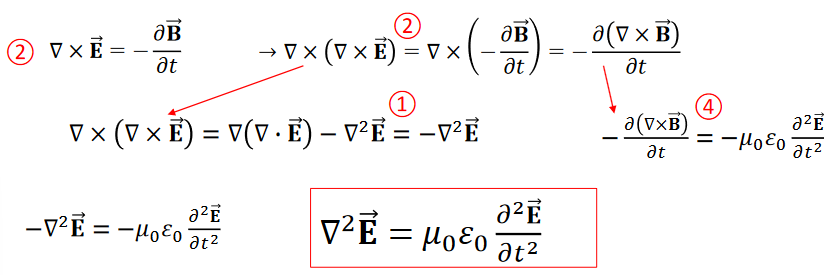
\includegraphics[width=0.5\textwidth]{screenshots/2024-04-16-11-39-34.png}
\end{figure}
Da questa equazione ricaviamo che \(c=\quotient{1}{\sqrt{\mu _0 \varepsilon _0} } \). Otteniamo lo stesso risultato per i vettori magnetici:
\begin{figure}[H]
	\centering
	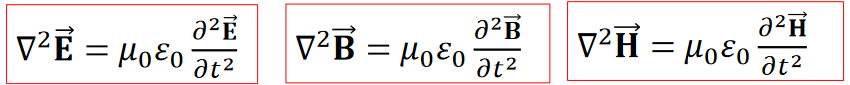
\includegraphics[width=0.6\textwidth]{screenshots/2024-04-16-11-42-01.png}
\end{figure}
Queste non sono tuttavia le equazioni delle onde elettromagnetiche! Da queste equazioni sembra che i campi siano indipendenti. Le onde elettromagnetiche sono descritte da equazioni che abbiamo già visto, ovvero le equazioni di Maxwell nel vuoto.

\paragraph{Onde elettromagnetiche piane armoniche}
Cerchiamo una soluzione nella forma di onde piane armoniche: \(\vec{E}(\vec{r},t)=\vec{E}_0 e^{i(\vec{k}\cdot \vec{r}- \omega t)},\ \vec{B}(\vec{r},t)=\vec{B}_{0} e^{i(\vec{k}\cdot \vec{r}-\omega t)}\). Sono onde in moto nella direzione \(\vec{k}\).
\begin{align}
	\frac{\partial \vec{E}}{\partial t}&= -i \omega \vec{E}_0 e^{i(\vec{k}\cdot \vec{r}-\omega t)}=-i \omega \vec{E} & \frac{\partial \vec{B}}{\partial t}=-i \omega \vec{B}  
\end{align}
\begin{figure}[H]
	\centering
	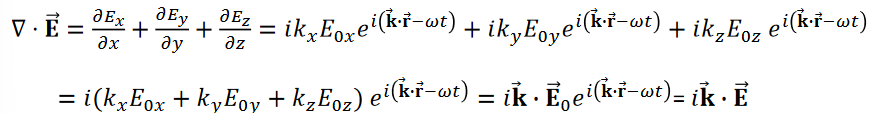
\includegraphics[width=0.7\textwidth]{screenshots/2024-04-16-11-49-51.png}
\end{figure}
Trattando queste onde, posso ricordarmi queste regole: \(\frac{\partial }{\partial t} = -i \omega,\ \div = i \vec{k}\cdot,\ \curl = i \vec{k} \cp,\ \grad = i \vec{k}\). Applicandole, ottengo che
\begin{figure}[H]
	\centering
	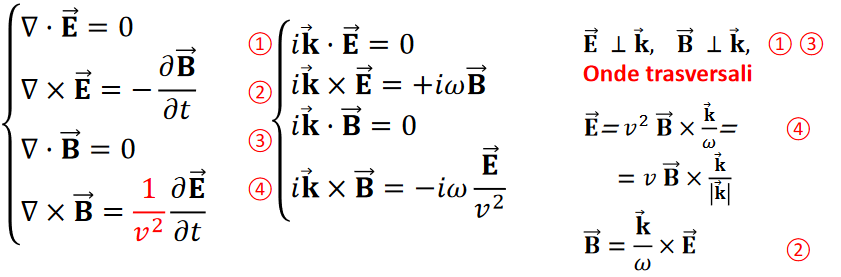
\includegraphics[width=0.6\textwidth]{screenshots/2024-04-16-11-54-38.png}
\end{figure}
Quindi \(\vec{E},\vec{B},\vec{k}\) costituiscono una terna destrorsa. Inoltre si ha che \(\vert \vec{E} \vert =v \vert \vec{B} \vert \). Queste sono condizioni che vanno rispettate anche da \(\vec{E}_0\) e \(\vec{B}_0\), quindi non possono avere qualsiasi valore.

Sia \(\vec{k}\) diretto come l'asse z (\(\vec{k}\cdot \vec{r}=kz\)). Quindi ho che 
\begin{figure}[H]
	\centering
	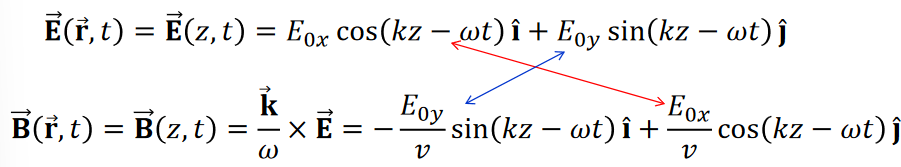
\includegraphics[width=0.6\textwidth]{screenshots/2024-04-16-12-02-43.png}
\end{figure}
La componente x di \(\vec{B}\) dipende dalla componente di y di \(\vec{E}\) e viceversa. Le onde si propagano come mostrato di seguito:
\begin{figure}[H]
	\centering
	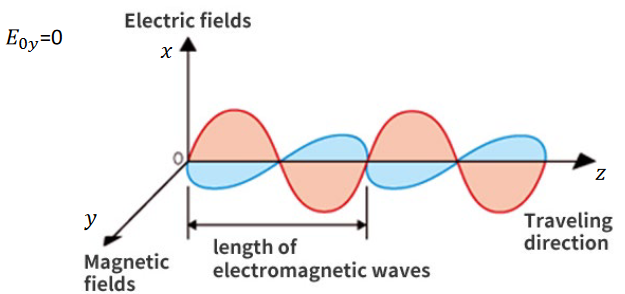
\includegraphics[width=0.4\textwidth]{screenshots/2024-04-16-12-04-04.png}
\end{figure}
I nodi sono nello stesso punto, sia per la parte magnetica che per la parte elettrica.

\section{Onde nei mezzi}
Nei mezzi non ci sono \(\mu _0\) e \(\varepsilon_0\), ma \(\mu\) e \(\varepsilon \). Quindi ho una velocità più bassa: \(v=\quotient{1}{\sqrt{\mu \varepsilon } } \). Se scrivo \(\vec{E}=v \vec{B}=v \mu \vec{H}\), noto che c'è una proporzionalità fra \(\vec{E}\) e \(\vec{H}\). Chiamo la costante di proporzionalità "impedenza elettromagnetica del mezzo". Rappresenta una relazione causa-effetto (come già visto)! Una variazione di \(\vec{E}\) produce una variazione di \(\vec{H}\).

\begin{definition}
	[Impedenza elettromagnetica]
	\begin{align}
		Z &= v \mu = \sqrt{\frac{\mu }{\varepsilon }} & 
		Z_0 &= c \mu _0 = \sqrt{\frac{\mu _0}{\varepsilon _0}}=\SI{377}{\ohm} 
	\end{align}
\end{definition}

\paragraph{Onde nei mezzi ottici}
Nei mezzi ottici \(\mu _r \thickapprox 1\) quindi \(v\thickapprox \quotient{c}{\sqrt{\varepsilon _r} } \).
\begin{definition}
	[Indice di rifrazione del mezzo]
	\begin{equation}
		n=\frac{c}{v}\geq 1,\ n \thickapprox \sqrt{\varepsilon _r} 
	\end{equation}	
\end{definition}
Di conseguenza
\begin{figure}[H]
	\centering
	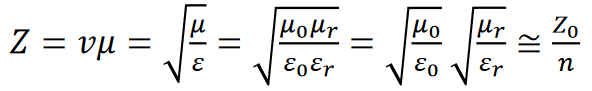
\includegraphics[width=0.4\textwidth]{screenshots/2024-04-16-12-13-57.png}
\end{figure}